\section{相关工作与文献综述}

文本情感分析（Sentiment Analysis）旨在从文本中自动抽取主观态度信息，是自然语言处理（NLP）的基础任务之一。随着社交平台与电商评论的规模不断膨胀，该技术已被广泛用于舆情监控、产品推荐等实际场景。从方法演进的角度看，情感分析经历了从手工规则、统计机器学习、深度学习，再到大语言模型的四个阶段。

\begin{figure}[htbp]
    \centering
    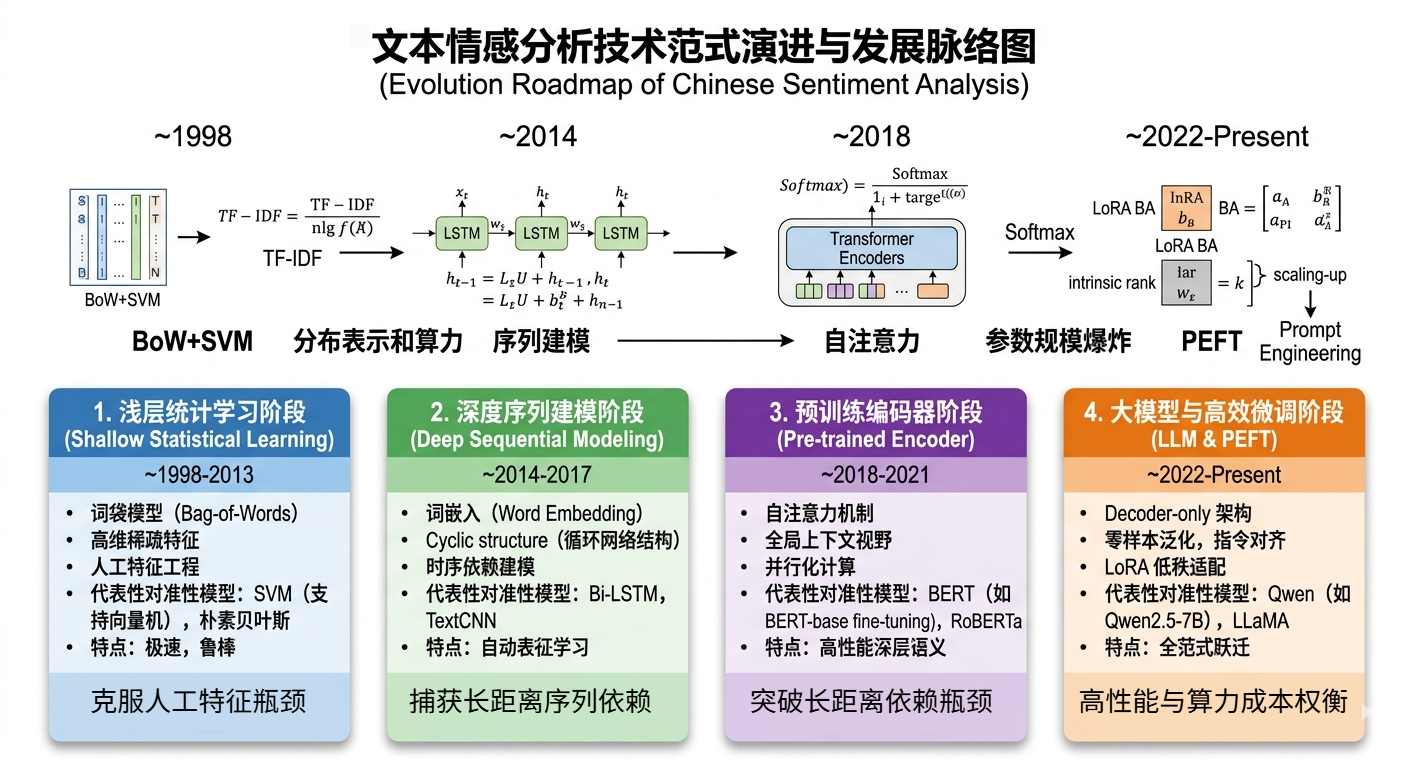
\includegraphics[width=0.95\textwidth]{figures/fig_timeline.png}
    \caption{中文情感分析技术发展脉络}
    \label{fig:timeline}
\end{figure}

\subsection{传统机器学习与特征工程}
在统计 NLP 的早期，研究者关注如何从文本中构造有区分力的特征。Joachims \cite{joachims1998text} 论证了 SVM 在处理高维稀疏文本时的优势——文本特征维度远高于样本量，而 SVM 通过寻找最大间隔超平面来抑制过拟合。
针对中文，Tan 等人 \cite{tan2008empirical} 在 ChnSentiCorp 等语料上发现，分词质量和特征选择方法（如 TF-IDF）对最终精度影响很大。但这类方法将文本视为词袋，丢掉了词序，遇到否定、反讽等需要通过上下文消歧的情况就容易出错。

\subsection{从序列建模到深度表示学习}
Word2Vec \cite{mikolov2013efficient} 把词映射为低维稠密向量，使语义计算成为可能。Kim \cite{kim2014convolutional} 用多尺度 CNN 做句子分类，验证了局部 n-gram 特征的有效性。
情感分析依赖长程上下文，因此 LSTM \cite{hochreiter1997long} 及其双向版本（Bi-LSTM）受到更多关注。Long 等人 \cite{long2019sentiment} 在 Bi-LSTM 上引入多头注意力，证明双向结构能同时编码前向与后向语义，提升了对长句情感逻辑的建模能力。不过 RNN 类模型是串行计算的，训练并行度低，当文本超过百词时梯度回传仍然吃力。

\subsection{预训练模型与 Transformer}
Vaswani 等人 \cite{vaswani2017attention} 提出自注意力机制，让任意两个词之间的信息通路不再受距离限制。Devlin 等人 \cite{devlin2018bert} 在此基础上设计了 BERT：用掩码语言模型在海量文本上预训练，再在下游标注数据上微调。BERT 及其改进版 RoBERTa \cite{liu2019roberta} 在情感分析等分类任务中长期占据最优位置。

\subsection{大语言模型与参数高效微调}
以 GPT 系列为代表的生成式大模型在少样本和零样本场景下展现出可观的泛化能力。Brown 等人 \cite{brown2020language} 探索了上下文学习（In-Context Learning）的潜力；Edwards 与 Camacho-Collados \cite{edwards2024language} 在 16 个分类数据集上做了系统对比，结论是：在标注数据可得的前提下，微调小模型往往优于大模型的少样本提示。
出于算力约束，参数高效微调（PEFT）日益受到重视。Hu 等人 \cite{hu2021lora} 提出的 LoRA 在冻结预训练权重的同时插入低秩旁路矩阵，将可训练参数量压缩到原模型的千分之一量级，使得在单卡 GPU 上微调 7B~13B 规模模型（如 Qwen 系列、LLaMA\cite{touvron2023llama}）变得可行。

\subsection{中文情感分析的特殊挑战}

上述方法大多在英文语料上验证后再迁移到中文场景，但中文情感分析面临一些独特困难，直接影响模型表现。

首先是分词歧义与粒度问题。中文没有天然的词边界，Jieba 等分词工具在不同场景下会给出不同切分结果。例如"武汉市长江大桥"可以被切分为"武汉/市长/江大桥"或"武汉市/长江/大桥"，前者改变语义、后者符合常识。当情感词的边界被错误切割——如"不舒服"被切成"不/舒服"是合理的，而"不是很好"若被切成"不是/很好"则丢失了"不"的否定作用——后续模型的特征提取就会出现偏差。

其次是组合式否定与程度修饰。中文的否定结构比英文复杂得多：双重否定（"不得不承认"）、三重否定（"并非不无道理"）、否定词与程度词的嵌套（"没有想象中那么好"、"不怎么好看"）等，都需要模型捕捉跨词甚至跨句的长程依赖。词袋模型（如 SVM 的 TF-IDF 特征）完全无法处理这种现象，它们将每个词独立对待，无法区分"好"与"不是很好"中"好"的语义差异。Bi-LSTM 虽然通过门控机制获得了序列建模能力，但在否定词与目标词相隔超过 10 个词时效果衰减明显 \cite{li2014improving}。

第三个挑战来自情感隐喻与反讽。中文用户常常用"打太极""画大饼""韭菜"等隐喻表达负面情感，字面义与情感完全无关。反讽句——如"这服务态度可真好，等了两个小时才有人理"——在字面上是正向词汇但整体表达是负面的，需要模块捕捉"等了两个小时"与"服务态度可真好"之间的矛盾。这类现象对模型的常识推理和语境理解提出了较高要求。

第四是网络语言与 OOV（Out-of-Vocabulary）问题。电商评论和社交平台中充斥着大量非规范表达："yyds""绝绝子""社死""破防了"等，它们更新速度快，通常不在预训练词表中。静态词嵌入（如 Word2Vec）和浅层模型对此束手无策，而 BERT 的子词切分机制（WordPiece）可以在一定程度上缓解——"绝绝子"被切为"绝/\#\#绝/\#\#子"后，模型仍可从"绝"的子词嵌入中提取正向信号。大语言模型则通过海量预训练语料覆盖了更多泛化表达。

最后是标注不一致与主观性。情感标注本质上带有主观色彩："还行"在有些人眼里是中性偏正，在另一些人眼里是中性偏负。ChnSentiCorp 等公开数据集在一定程度统一了标注标准，但边缘样本的混淆仍是所有模型面临的共性问题。

\subsection{本研究的定位与动机}

综合来看，各技术路线的精度在持续提高，但工程上选择哪种模型不能只看精度。现有的英文基准评测研究（如 GLUE、SuperGLUE）已较为充分，但中文情感分析场景下缺少在同一数据集和同一计算环境中将统计学习、深度序列建模、预训练编码器与大语言模型进行系统对比的工作。本研究的出发点就是：在统一的实验条件下，对 SVM、Bi-LSTM、BERT、Qwen 等代表性方法做横向对比，不仅比较精度，还纳入训练成本、推理延迟和参数规模等因素，为模型选型提供量化的参考。
